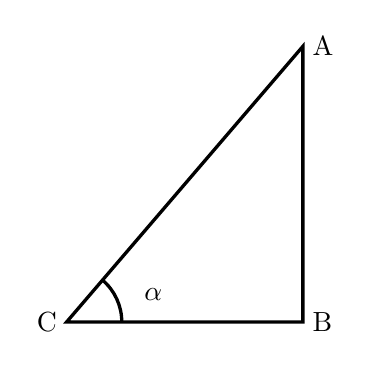
\begin{tikzpicture}[scale=1]

  % Define the vertices of the right-angled triangle
  % Adjusting coordinates to match the approximate proportions of the image
  \coordinate (C) at (0,0);
  \coordinate (B) at (3,0);
  \coordinate (A) at (3,3.5);

  % Draw the thick lines of the triangle
  \draw[very thick] (C) -- (B) -- (A) -- cycle;

  % Draw the arc for angle alpha at vertex C
  % The angle is approximately atan(3.5/3) = 49.4 degrees
  \draw[very thick] (0.7,0) arc (0:49.4:0.7);

  % Add the label for angle alpha inside the arc
  \node at (1.1, 0.35) {$\alpha$};

  % Add the labels for the vertices exactly where they appear in the image
  \node[left] at (C) {C};
  \node[right] at (B) {B};
  \node[right] at (A) {A};

\end{tikzpicture}